\documentclass[a4paper,12pt]{report}
\usepackage{amsmath,amsfonts,amssymb,enumerate,graphicx,fancyhdr,times}
\usepackage{tabularx,float,xspace,float,caption,setspace}
\usepackage[top=1in, left = 1.3in, right = 1in, bottom = 0.8in]{geometry}
\usepackage[utf8]{inputenc}

\pagestyle{fancyplain}
\fancyhf{}
\renewcommand{\headrulewidth}{0px}
\fancyfoot[R]{\thepage}
\parindent 0px

\begin{document}

\begin{titlepage}

	\centering

	
\includegraphics[width=3cm, keepaspectratio]{cuet.png} \par \vspace{0.5cm}
	\begin{Large}
		CHITTAGONG UNIVERSITY OF ENGINEERING \& TECHNOLOGY
	\end{Large}
	\par
	\vspace{.5cm}
	{DEPARTMENT OF COMPUTER SCIENCE AND ENGINEERING}
\vspace{1cm}

	\raisebox{-\baselineskip}{\rule{\textwidth}{1px}}
	\rule{\textwidth}{1px}

\vspace{0.2cm}
{\large{{EXPERIMENT NAME}}}\par \vspace{0.3cm}
\Large{{Completion of other pages and  database of ``SmartHaat" Website.}}
	\rule{\textwidth}{2px}

\vspace{0.5cm}

	\normalsize
\begin{tabular}{cl}
COURSE CODE        & : CSE 326                          \\
COURSE NAME        & : INTERNET PROGRAMMING (SESSIONAL) \\
EXPERIMENT NO      & : 06                               \\
DATE OF SUBMISSION & : 02 -- 08 -- 2023
\end{tabular}
\vspace{0.5cm}

	\parbox[l]{9cm}{
		\begin{center}
			submitted by
		\end{center}

		\begin{tabular}{cl}
			MD AKIB HASAN        & $(1904015)$ \\
K.M. MAHABUB HOSSAIN & $(1904017)$ \\
			SADMAN RAHMAN ANANTA & $(1904020)$ \\
		\end{tabular}
	}
	\parbox[r]{6cm}{
		\vspace{1cm}
		\begin{center}
			
\includegraphics[width=4cm, keepaspectratio]{remarks.png}
			\captionof*{figure}{REMARKS}
		\end{center}
	}

	\vspace{0.5cm}
	supervised by

	\parbox[l]{7.5cm}{\begin{center}

			SABIHA ANAN\\
\footnotesize{Assistant Professor\\
				Department of CSE, CUET}
		\end{center}
	}
	\parbox[r]{7.5cm}{\begin{center}

			MD RASHADUR RAHMAN\\
\footnotesize{Lecturer \\
				Department of CSE, CUET}
		\end{center}
	}

	\vfill
\end{titlepage}


\onehalfspacing

\section*{Experiment Name}
Completion of other pages and  database of ``SmartHaat" Website.
\section*{Objectives}
\begin{itemize}
\item Creating firm, wishlist, butchers pages.
\item Adding firm registration, post upload etc. form.
\item Implementing payment system.
\end{itemize}
\section*{Description}
A websites compatibility and efficiency depends on quick response to the user and providing them hassle-free service as well as sellers. Therefore, we implemented pages not only containing sellers but also firms. Because, customers could easily trust well known firms. 
\begin{figure}[H]
\centering
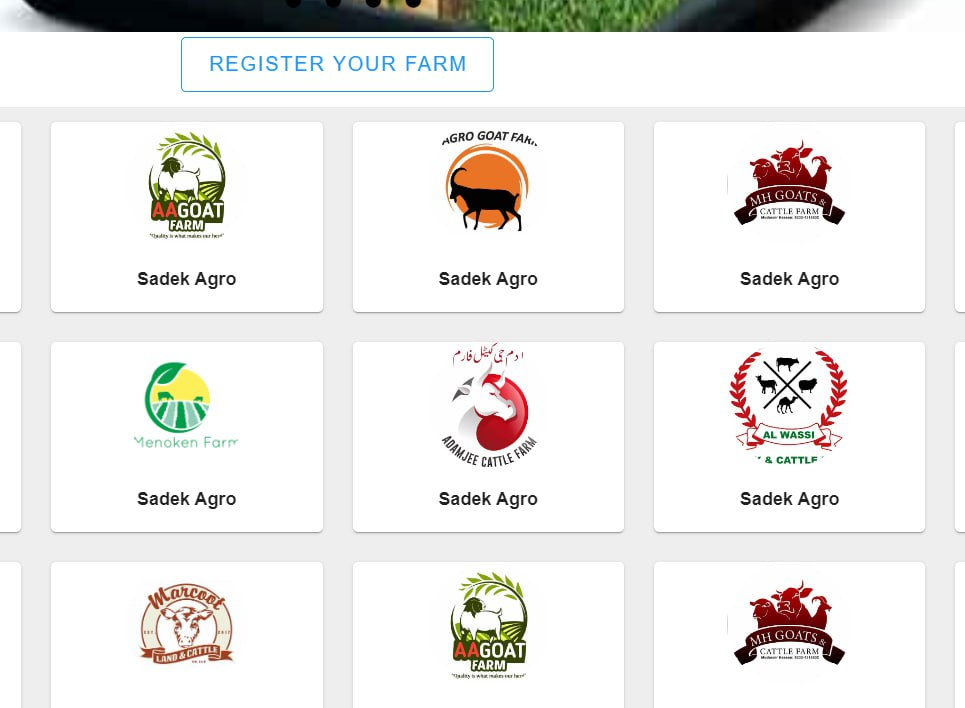
\includegraphics[keepaspectratio, width=12cm]{firm.jpg}
\caption{Firms page}
\label{firms}
\end{figure}

As we can see in the figure \ref{firms} shows the list of firms. Therefore, we also implemented a system where users can register their farms. With necessary information, a firm can be registered and after verification it can be displayed.
\begin{figure}[H]
\centering
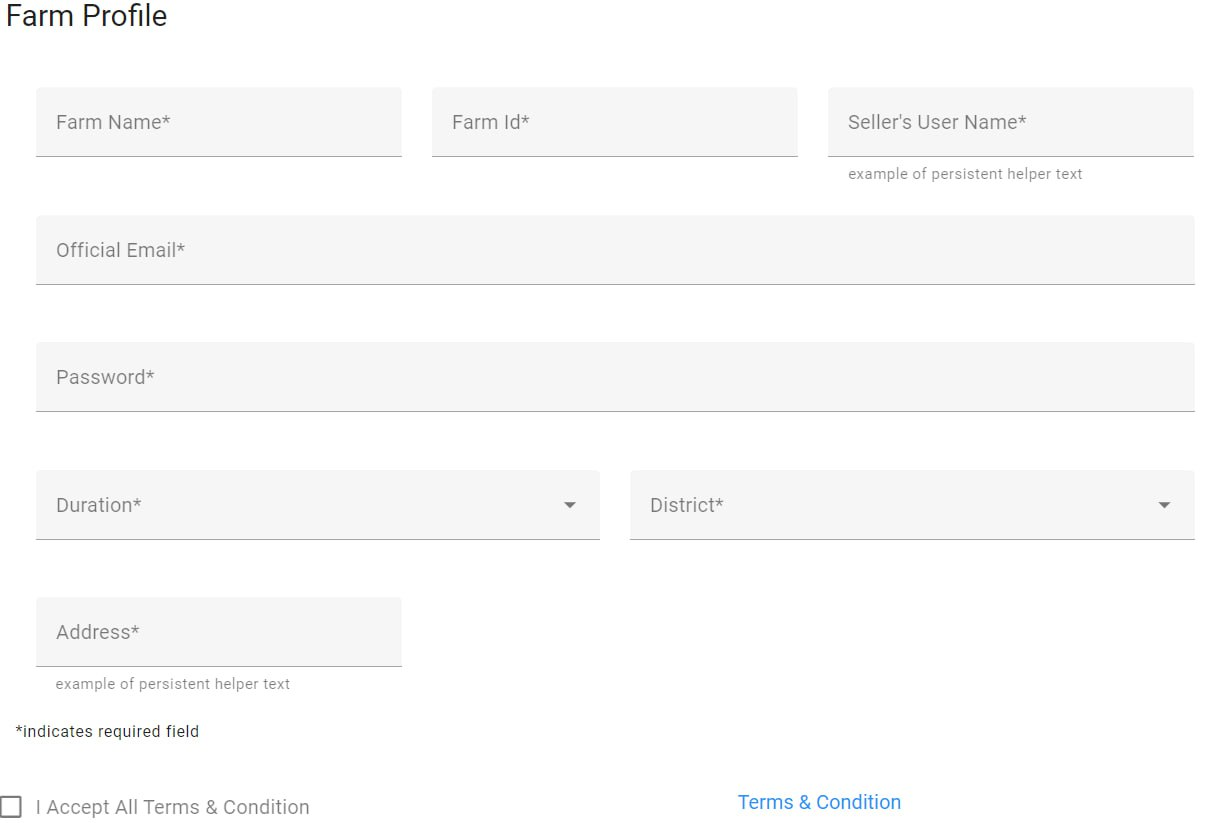
\includegraphics[keepaspectratio, width=12cm]{reg-firm.jpg}
\caption{Firms registration page}
\label{firms-reg}
\end{figure}
An important feature of ``SmartHaat'' website is butcher supplying system, where users can order butchers on their desired times.
\begin{figure}[H]
\centering
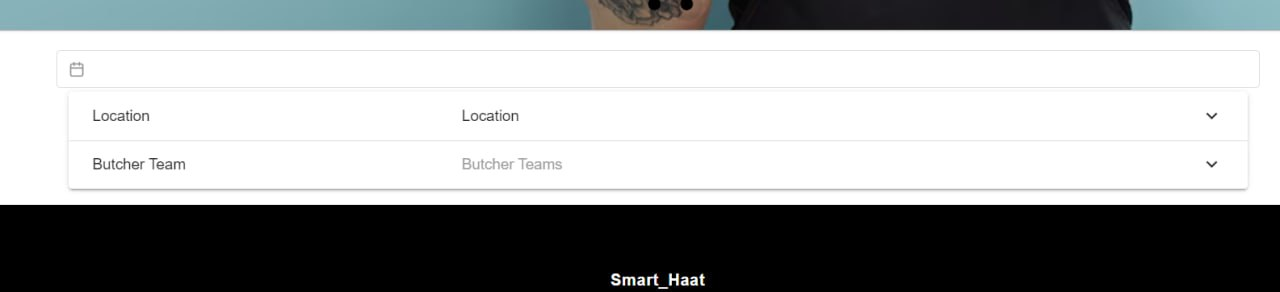
\includegraphics[keepaspectratio, width=12cm]{butcher.jpg}
\caption{Butcher page}
\label{butcher}
\end{figure}
Here, butcher is supplied using the nearest location possible and free time is also a necessary condition. After these conditions are met by user, we can provide butchers.
\begin{figure}[H]
\centering
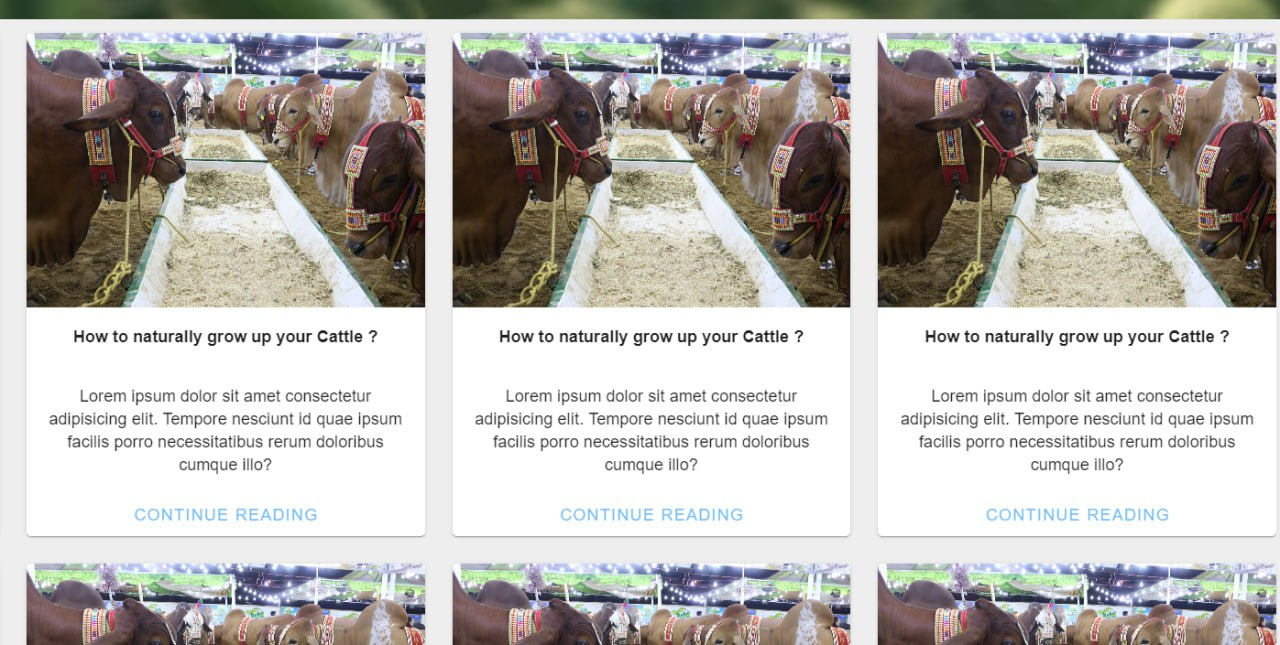
\includegraphics[keepaspectratio, width=12cm]{blog.jpg}
\caption{Blog post page}
\label{blog}
\end{figure}

One of the unique feature of our website was blogging system, where we could incorporate good writings of various scholars on different regards. Following figure \ref{blog} offers similar kind of feature.


In order to add post there is a post submitting page. In figure \ref{post} it shows an inner view of blog posts where digital media such as videos, audios images as well as text can be added.
\begin{figure}[H]
\centering
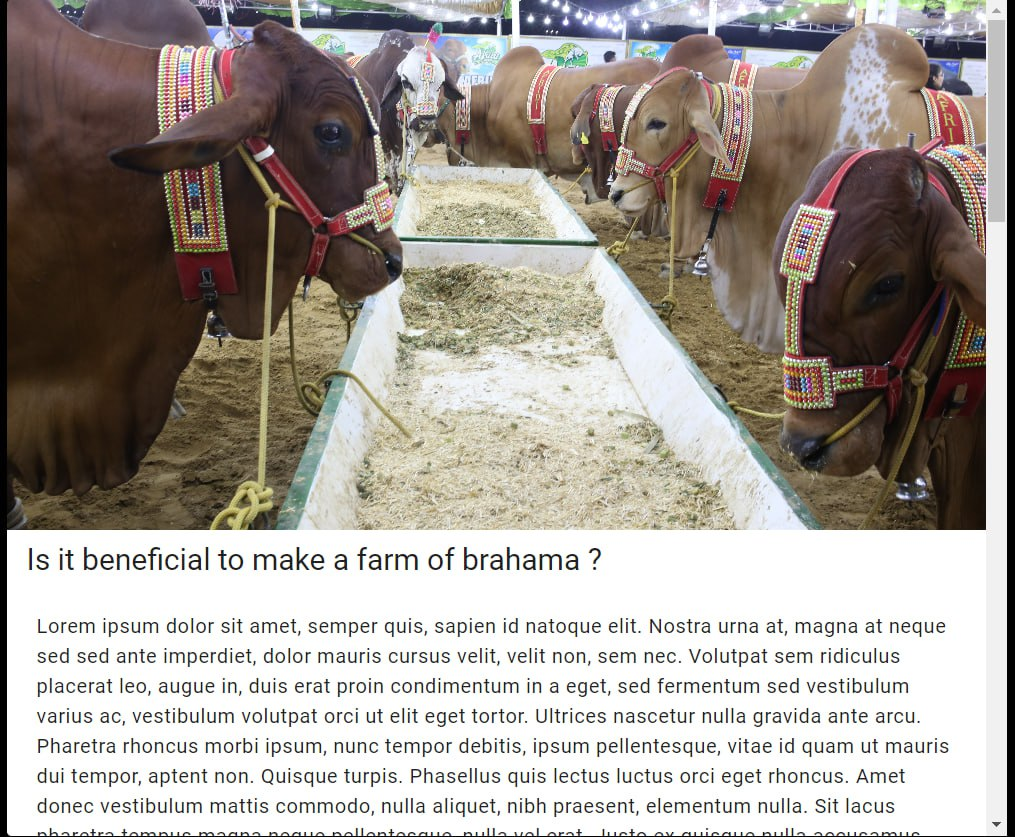
\includegraphics[keepaspectratio, width=12cm]{blogpost.jpg}
\caption{Inner blog post page}
\label{post}
\end{figure}

There is a wishlist page where a product can be saved which can be further be added to cart and order. The wishlist page is shown in figure \ref{wlst}, where it has product details, add to cart option and remove option.
\begin{figure}[H]
\centering
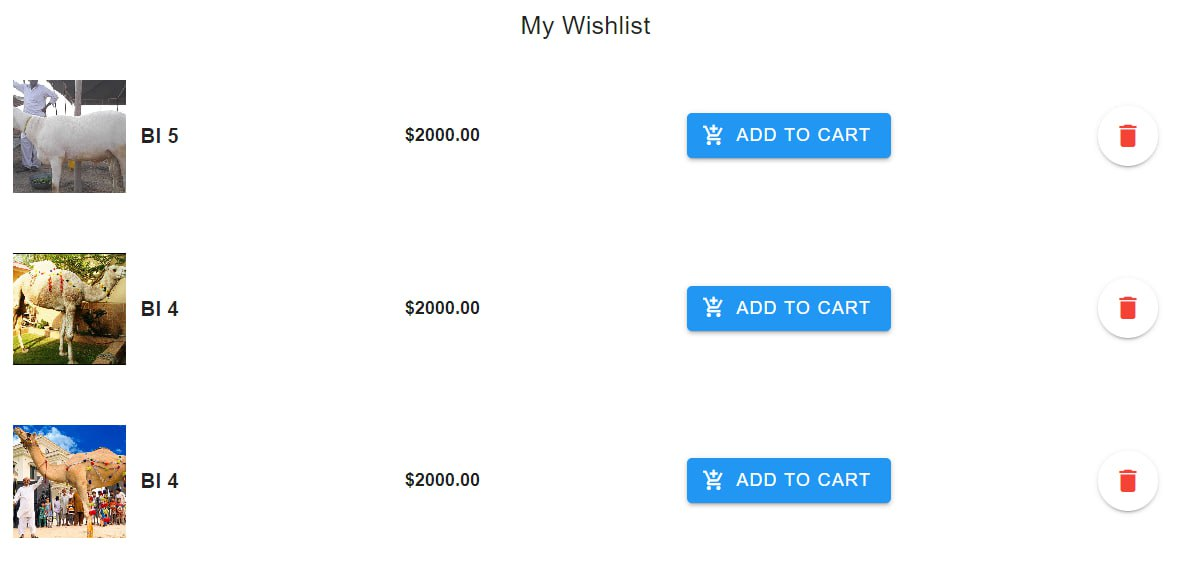
\includegraphics[keepaspectratio, width=12cm]{wishlist.jpg}
\caption{Wishlist page}
\label{wlst}
\end{figure}

Finally, a good and reliable payment system can make an e-commerce website more complete. Thus, we've incorporated a payment system where COD and card payment available which are shown in figure \ref{pmnt}.
\begin{figure}[H]
\centering
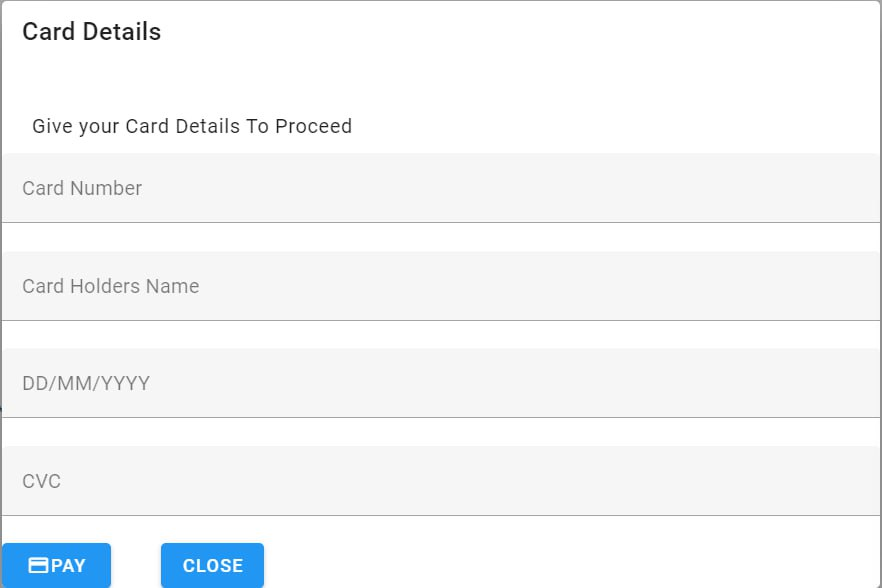
\includegraphics[keepaspectratio, width=12cm]{payment.jpg}
\caption{Payment page}
\label{pmnt}
\end{figure}

With necessary information payment is available through our website.

There are more basic features we've added such as login system, improved cart and others. Also, some defects were fixed too.





\section*{Development Platforms}
The frameworks and language platforms we used --
\begin{itemize}
	\item HTML
	\item CSS
\item JavaScript
	\item VUE
\item Django REST API
\item Sqlite3
\end{itemize}

\section*{Conclusion}
``SmartHaat'' website offers a basic kind of e-commerce experience with some special features on am unique concept. The main goals were to provide the users expected features in a modern UI. Therefore, easy and quick responsive pages are built for our website.

This week we improved various pages with more functionalities and features. The payment page took a bit of difficulty, but it was solved finally. And there are also some small unfinished tasks which could be solved. Some data can't be accessed without proper APIs and that's why some functions are not available.
There are some server issue for which some parts don't work sometimes which also solved after many attempts.
\end{document}
